\begin{pastexam}[label={px:gw3-096-ds-03}]{關務三等資訊處理 96 年 第三題}
（申論；20 分）

以下為前序追蹤（Preorder Traversal）及後序追蹤（Postorder Traversal）的順序\\
前序追蹤順序：M, N, I, A, H, B, C, J, G, F, K, L, E, D, Y\\
後序追蹤順序：A, B, C, H, I, G, F, J, N, E, D, L, Y, K, M
\begin{itemize}[leftmargin=2.2em, nosep]
\item[㈠] 請畫出此二元樹。（10 分）
\item[㈡] 請寫出此二元樹的中序追蹤（Inorder Traversal）順序。（10 分）
\end{itemize}
\end{pastexam}

\begin{pastsoln}
答案：㈠ 樹畫在下面（唯一）。 ㈡ A, I, B, H, C, N, G, J, F, M, E, L, D, K, Y。

\textbf{㈠ 重建}（資結書第~7.4~節）：前序第一個、後序最後一個是根。 根之後前序的下一個是左子樹的根 $a$；在後序裡找到
$a$，$a$ 和它前面的部分就是左子樹，其餘（扣掉最後的根）是右子樹。
\begin{itemize}
\item 根 $M$。 前序下一個 $N$，在後序第 $9$ 個，所以左子樹有 $9$ 個節點：前序 N I A H B C J G F、後序
A B C H I G F J N；右子樹前序 K L E D Y、後序 E D L Y K。
\item $N$：左子樹根 $I$，後序第 $5$ 個：前序 I A H B C、後序 A B C H I；右子樹前序 J G F、後序 G F J。
\item $I$：左子樹根 $A$，後序第 $1$ 個，只有 $A$；右子樹前序 H B C、後序 B C H，是 $H$ 帶左子 $B$、右子 $C$。
\item $J$：前序 G F、後序 G F，左子 $G$、右子 $F$。
\item $K$：左子樹根 $L$，後序 E D L 共 $3$ 個，是 $L$ 帶左子 $E$、右子 $D$；右子樹只有 $Y$。
\end{itemize}
\begin{center}
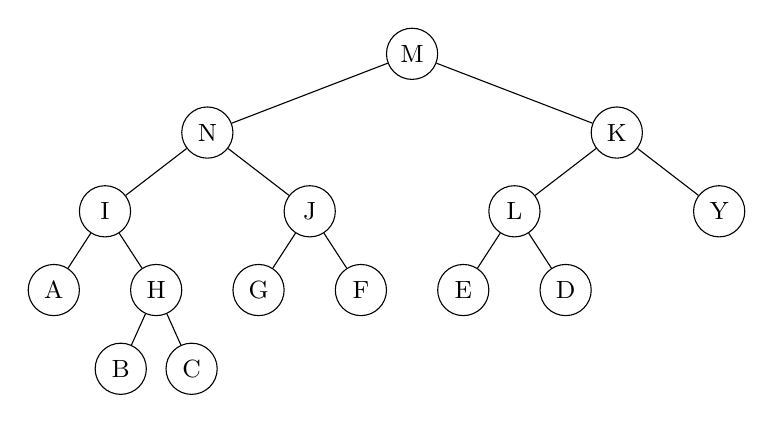
\begin{tikzpicture}[every node/.style={circle,draw,minimum size=6.5mm,inner sep=0pt,font=\small},
  level distance=10mm, level 1/.style={sibling distance=52mm}, level 2/.style={sibling distance=26mm},
  level 3/.style={sibling distance=13mm}, level 4/.style={sibling distance=9mm}]
\node {M}
  child {node {N}
    child {node {I} child {node {A}} child {node {H} child {node {B}} child {node {C}}}}
    child {node {J} child {node {G}} child {node {F}}}}
  child {node {K}
    child {node {L} child {node {E}} child {node {D}}}
    child {node {Y}}};
\end{tikzpicture}
\end{center}
\textbf{唯一性。} 前序加後序一般不能決定二元樹：只有一個子節點的節點，看不出子節點在左或在右（資結書定理~7.5，符合的
樹有 $2^{k}$ 棵，$k$ 是只有一個子節點的節點數）。 這裡每一步拆出的左右子樹都不空，內部節點 $M, N, I, H, J, K, L$ 都
恰有兩個子節點，$k = 0$，所以樹是唯一的。

\textbf{㈡ 中序}（左、根、右）：$I$ 子樹是 A I B H C，$J$ 子樹是 G J F，所以 $N$ 子樹是 A I B H C N G J F；$K$ 子樹是
E L D K Y。 整棵樹：
\[
A, I, B, H, C, N, G, J, F, M, E, L, D, K, Y.
\]
\end{pastsoln}
